\documentclass{article}

% if you need to pass options to natbib, use, e.g.:
%     \PassOptionsToPackage{numbers, compress}{natbib}
% before loading neurips_2021

% ready for submission
\usepackage[final]{neurips_2021}

% to compile a preprint version, e.g., for submission to arXiv, add add the
% [preprint] option:
%     \usepackage[preprint]{neurips_2021}

% to compile a camera-ready version, add the [final] option, e.g.:
%     \usepackage[final]{neurips_2021}

% to avoid loading the natbib package, add option nonatbib:
%    \usepackage[nonatbib]{neurips_2021}

\usepackage[utf8]{inputenc} % allow utf-8 input
\usepackage[T1]{fontenc}    % use 8-bit T1 fonts
\usepackage{hyperref}       % hyperlinks
\usepackage{url}            % simple URL typesetting
\usepackage{booktabs}       % professional-quality tables
\usepackage{amsfonts}       % blackboard math symbols
\usepackage{nicefrac}       % compact symbols for 1/2, etc.
\usepackage{microtype}      % microtypography
\usepackage{xcolor}         % colors
\usepackage{amsmath}
\usepackage{algorithm}      % algorithms
\usepackage{algpseudocode}  % algorithms
\usepackage[english]{babel} % citations
\usepackage{natbib}         % citations
\usepackage{dirtytalk}      % quotations
\usepackage{graphicx}
\bibliographystyle{abbrvnat}
\setcitestyle{numbers,open={[},close={]}} %Citation-related commands

\title{Single-Encoder VAE Image-To-Image Translation}

% The \author macro works with any number of authors. There are two commands
% used to separate the names and addresses of multiple authors: \And and \AND.
%
% Using \And between authors leaves it to LaTeX to determine where to break the
% lines. Using \AND forces a line break at that point. So, if LaTeX puts 3 of 4
% authors names on the first line, and the last on the second line, try using
% \AND instead of \And before the third author name.

\author{%
  Adit Gajjar
  % \thanks{Use footnote for providing further information
  %   about author (webpage, alternative address)---\emph{not} for acknowledging
  %   funding agencies.}
  \\
%   University of Toronto\\
  % Cranberry-Lemon University\\
  % Pittsburgh, PA 15213 \\
  % \texttt{hippo@cs.cranberry-lemon.edu} \\
  % examples of more authors
  \And
  Harsh Nasit \\
%   University of Toronto\\
  % Address \\
  % \texttt{email} \\
  \And
  Filip Balucha \\
%   University of Edinburgh\\
  % Address \\
  % \texttt{filip.balucha@mail.utoronto.ca} \\
}

\begin{document}

\maketitle

% TODO: remove line numbers?
\begin{abstract}
  Image-to-image translation is a computer vision problem where an image is mapped from one domain to another. In the supervised scenario, the dataset consists of perfectly-paired image data. However, such data is either hard to find or simply does not exist \citep{zhu}. Therefore, we focus on the unsupervised setting, where a joint distribution of images across two domains is learnt using the marginal distributions – the images in individual domains \citep{liu}. We propose a model that builds on the shared latent space assumption and uses domain-specific decoders. In addition, our approach readily extends to more than two different domains. The implementation is available at https://github.com/HareshNasit/CSC413-Project.
\end{abstract}
\section{Introduction}
At a high level, image-to-image translation aims to capture the characteristics of one image collection and determine how these could be translated into another image collection \citep{zhu}. Mathematically, the goal is to learn a mapping $G: X \rightarrow Y$, where X is the source and Y the target domain.

Image-to-image translation includes many computer vision problems, such as super-resolution, colorization and style transfer \citep{liu}. Style transfer has various applications in photo and video editing, customized gaming styles and commercial art. Transfering styles between images is a hard image processing task because it is difficult to represent semantic information such as image texture.

Many efforts were put into the supervised setting, where models learn image-to-image translation across two domains using perfectly-paired images \citep{zhu}. However, obtaining paired data is often difficult and expensive, and sometimes impossible \citep{zhu}. For example, to learn the translation from photographs to images styled as Monet paintings, the supervised setting would require pairs of real-life images and the corresponding Monet paintings – an infeasible task. Therefore, we focus on unsupervised algorithms that map between domains without paired examples.

From a probabilistic perspective, the aim is to learn a joint distribution of images between two different domains, where each domain consists of images from a marginal distribution \citep{liu}. However, there are infinitely many such joint distributions \citep{liu}. To address this problem, we can add more structure to the objective \citep{zhu} or make assumptions about the structure of the joint distribution \citep{liu}.

For example, the CycleGAN model resolves this by training two mappings $G: X \rightarrow Y$ and $F: Y \rightarrow X$, and updating the objective to enforce $F(G(x)) \approx x$ and $G(F(y)) \approx y$ \citep{zhu}. By contrast, \citet{liu} assume a shared latent space, where a pair of corresponding images from different domains is mapped to the same latent representation.

Inspired by the stable training and meaningful encodings characteristic of variational autoencoder (VAE) models, we continue in the latter vein. We propose a model that leverages the shared latent space assumption but is simpler than the model proposed by \citet{liu}. While our model does not outperform theirs, we propose future directions that could bring our architecture to fruition.

\section{Related works}
 Image-to-image translation is a well-studied problem. We provide a summary of papers that tackle the unsupervised setting. We focus on two well-known architectures – the popular Generative Adversarial Networks (GANs) and the Variational Autoencoders (VAEs), praised for learning useful representations that lend themselves to manipulation.

\textbf{GANs.} CycleGAN builds on the successful GAN architecture by introducing cycle-consistency. This constrains the image-to-image translation problem and encourages meaningful translations \citep{zhu}.

\textbf{VAEs.} Several methods use VAEs in the context of image-to-image translation or style transfer. ST-VAE performs multiple style transfer by projecting styles to a linear latent space and merging them using linear interpolation \citep{liu2}. \citet{kazemi} propose a framework that explicitly models two representations – one for image content and another for style. \citet{larsen} propose VAE-GAN, which combines a VAE and the discriminator from the GAN architecture. Finally, \citet{jha} apply the cycle-consistency idea to the VAE setting.

\textbf{VAEs and Shared latent representation.} Several research efforts establish a shared latent space. \citet{zhao} propose a mapping between the two latent spaces corresponding to the two domains. Perhaps closest to our approach, \citet{liu} share the latent space z between the two domains by sharing some weights of domain-specific encoders and decoders. Our simplified architecture achieves the same using a single, shared encoder.

\section{Method}
\subsection{Objective}
The objective adapts the vanilla VAE objective that consists of a variational and a reconstruction term.
\subsubsection{Variational loss}
The variational loss term regularizes the latent space. It captures the KL divergence between the approximated posterior and the prior distribution. The posterior represents the \say{encoder} distribution, and the prior represents the family of distribution the encoder distribution should belong to. Similar to the original VAE paper, we assume both of these distributions are Gaussian \citep{kingma}. This allows us to express the variational loss term as
\begin{equation}
  \mathcal{L}_{\text{Variational}}
    = \frac{1}{\left|\mathcal{B}\right|} \sum_{i \in \mathcal{B}} \sum_{j=1}^J \left(
      1
      + \log\left(
        \left(
          \sigma_j^{(i)}
        \right)^2
      \right)
      - \left(\mu_j^{(i)}\right)^2 
      - \left(\sigma_j^{(i)}\right)^2 
    \right)
\end{equation}
where $\sigma$ and $\mu$ determine the approximated \say{encoder} distribution, $J$ is the latent dimension, and $i$ ranges over all samples in the batch $\mathcal{B}$.
\subsubsection{Reconstruction loss}
The original VAE paper uses a MSE reconstruction loss function \citep{kingma}. However, in the context of images, this loss function assumes that the impact of noise is independent of the local characteristics \citep{zhao2}. We therefore use a multiscale structural similarity index (MS-SSIM) term. MS-SSIM is a differentiable similarity metric that takes into account local features at various scale \citep{zhao2} and aims to produce visually-pleasing outputs. However, we found that using MS-SSIM term alone led to slow convergence. Therefore, similar to \citet{zhao2}, we instead augment the original MSE loss with MS-SSIM. We therefore express the reconstruction loss as
\begin{equation}
  \mathcal{L}_{\text{Reconstruction}}
    = \frac{1}{\left|\mathcal{B}\right|} \sum_{i \in \mathcal{B}}
    \text{MSE}\left(
      \mathbf{u}^{(i)},
      \mathbf{\tilde{u}}^{(i)}
    \right)
    + \text{MS-SSIM}\left(
      \mathbf{u}^{(i)},
      \mathbf{\tilde{u}}^{(i)}
    \right)
\end{equation}

\subsubsection{Full loss}
Finally, our full objective can be expresses as
\begin{equation}
  \mathcal{L}
  = \mathcal{L}_{\text{Variational}}
  + \alpha\cdot \mathcal{L}_{\text{Reconstruction}}
\end{equation}
where $\alpha$ is used to account for different learning rates between the two loss terms.
\subsection{Architecture}
\textbf{Training 1: Encoder.} Our architecture combines the components of the standard convolutional VAE (Figure \ref{fig:pretrain}). Both domains share a single encoder $E$, which is trained in concord with a shared decoder $D$. Its purpose is to establish a shared latent space where, based on the shared latent space assumption, images with similar content from different domains will be mapped to a similar point.
\begin{figure}[H]
  \centering
  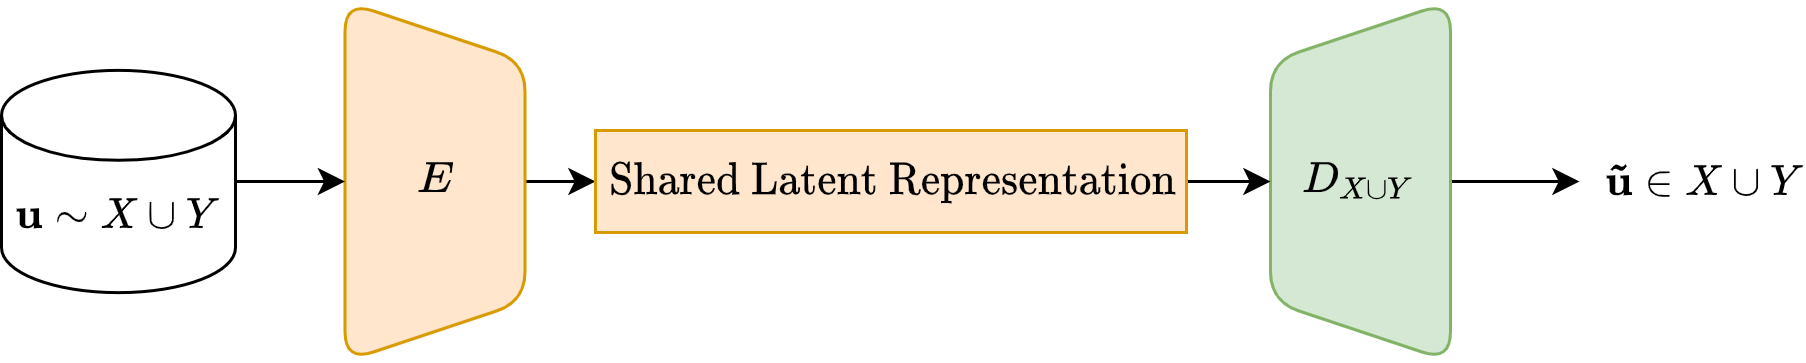
\includegraphics[width=0.7\linewidth]{report/assets/pretrain.png}
  \caption{Learning a shared latent representation for both image domains.}
  \label{fig:pretrain}
\end{figure}
\begin{algorithm}[H]
  \caption{The pre-training procedure}\label{alg:pre-train}
  \begin{algorithmic}
    \State{// $X, Y \gets \text{loadDataset}()$}
    \State{$M \gets \text{new VAE}()$}
    
    \State{$E \gets \text{new Encoder}()$}
    \State{$M\text{.encoder} \gets E$}
    
    \State{$D \gets \text{new Decoder}()$}
    \State{$M\text{.decoder} \gets D$}
    
    \State{$M\text{.train}(X \cup Y)$}
    
  \end{algorithmic}
  \end{algorithm}

\textbf{Training 2: Domain-specific decoders.} Once the encoder is trained, the encoder weights are frozen to fix the mapping to a shared latent space. Then, a separate decoder is trained for each domain (Figure \ref{fig:train}). For example, if we wish to map between images of apples and oranges, $E$ would encode images of both, apples and oranges, and there would be a dedicated decoder for each apples and oranges, respectively. 
\begin{figure}[H]
  \centering
  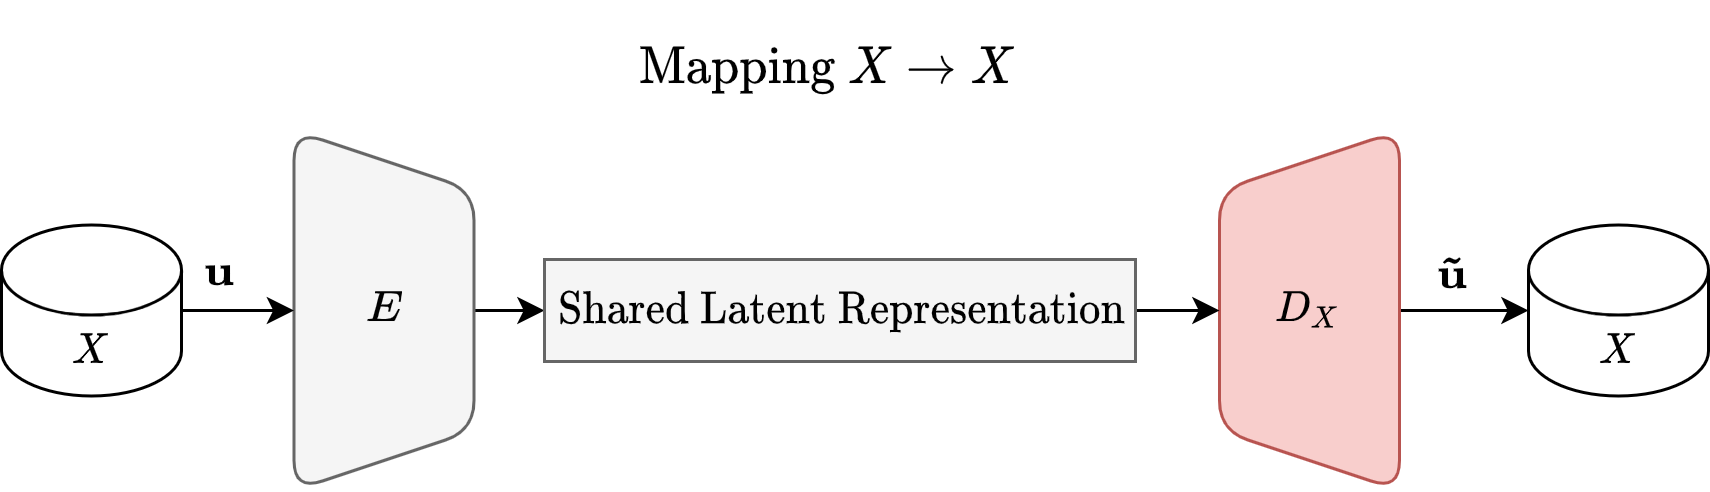
\includegraphics[width=0.7\linewidth]{report/assets/train.png}
  \caption{Learning the decoder $D_X$ for domain $X$ that uses embeddings from the shared latent space.}
  \label{fig:train}
\end{figure}
% \begin{algorithm}[H]
%   \caption{The training procedure}\label{alg:train}
%   \begin{algorithmic}
%     \State{// $X, Y \gets \text{loadDataset}()$}
%     \State{$D_X \gets \text{new Decoder}()$}
%     \State{$M\text{.decoder} = D_X$}
    
%     \State{$M$.encoder.freeze()}
    
%     \State{$M\text{.train}(X)$}
%     \end{algorithmic}
% \end{algorithm}

\textbf{Style transfer.} To perform style transfer, we simply combine the encoder $E$ and a domain-specific decoder $D_X$ or $D_Y$. For example, to obtain a mapping from domain $Y$ to $X$, it suffices to use the encoder E and decoder $D_X$ (Figure \ref{fig:eval}).

\begin{figure}
  \centering
  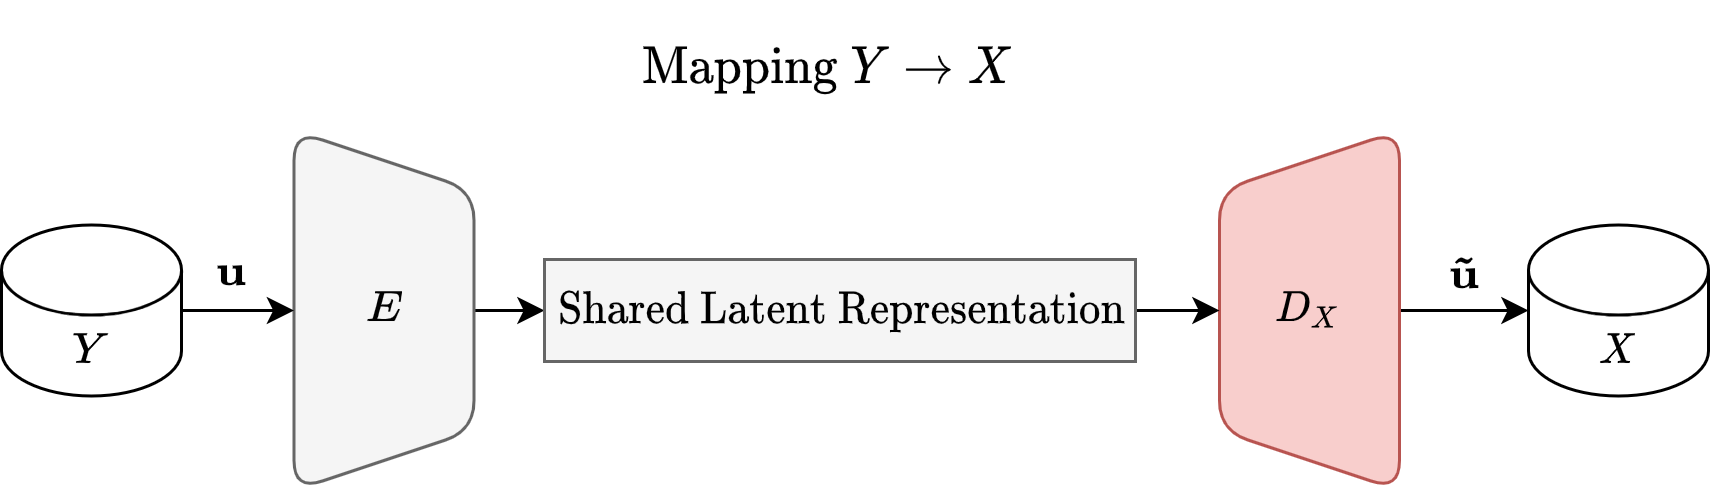
\includegraphics[width=0.7\linewidth]{report/assets/eval.png}
  \caption{Performing style transfer from domain $Y$ to $X$ using the shared encoder $E$ and domain-specific decoder $D_X$.}
  \label{fig:eval}
\end{figure}
% \begin{algorithm}[H]
%   \caption{The evaluation procedure}\label{alg:eval}
%   \begin{algorithmic}
%     \State{$M\text{.predict}(y \sim Y)$}
%   \end{algorithmic}
% \end{algorithm}

\section{Experiments}
We performed image translation experiments using three different datasets. The hyperparameters used to train on all the datasets can be found in Table \ref{tab:hyperparams}. The model results in translations that have some characteristics of the target domain, but the outputs still have blurry edges and lack clarity.
\subsection{\texttt{apple2orange}}
Our model's performance on \texttt{apple2orange} dataset was promising as it learnt the shape and color of the fruits well. For instance, in the below translation of orange to apple, the translation removed the leaf and the stem of the orange. Qualitatively, the translations of orange to apple look better than vice versa.

\subsection{\texttt{summer2winter\_yosemite}}
Our model's performance on \texttt{summer2winter\_yosemite} was not as good as \texttt{apple2orange} dataset. Qualitatively, we can tell the difference between the translations of the two seasons. The model learnt the color of the sky and the trees. The translations of summer images to winter resulted in output images that had gray skies and black trees, vice versa, the outputs had blue skies and green trees.

\subsection{\texttt{horse2zebra}}
Our model performed the worst on the \texttt{horse2zebra} dataset. Qualitatively, it is impossible to tell the difference between the translations of the two animals – the translations only show the silhouette. It is possible that the model was not able to learn the physical features of the two animals since the horse dataset consists of horses of multiple colors.

% TODO: figure

% \subsection{Evaluation metrics}

% \subsection{Limitations}

\section{Conclusion and future work}
Our VAE architecture performs worse than CycleGAN or the related architecture proposed by \citet{liu}. While the output content (e.g. the rough horse and zebra silhouettes) is maintained, the output quality is subpar. Our domain-specific decoder was likely limited by the quality of the latent representation produced by the shared encoder.

A more complex encoder, such as the one proposed by \citet{liu}, could learn a better representation of the domains and thus produce better translations. Another way to produce higher-quality images would be to replace our standard VAE architecture with a hierarchical VAE or VQ-VAE which has been shown to produce higher quality reconstructions. In addition, a more-informed loss function could improve quality. For instance, similar to \citet{liu}, a loss term based on a discriminator network could be used for translated images.

\newpage
\bibliography{sample}

\newpage
\appendix
\section*{Appendix}
\renewcommand{\thesubsection}{\Alph{subsection}}
\subsection{Training details}
\subsubsection{Layer dimensions}
The shared encoder E and the domain-specific decoders $D_x$ and $D_y$ have the same size. Both the encoder and decoders are 5-layer deep with the following hidden sizes: 32, 64, 128, 256 and 512. The latent representation was a 256-dimensional vector. Each encoder and decoder layer included, in sequence, a convolution or transposed convolution, batch normalization, and the Leaky ReLU activation function. We use the Adam optimizer with a batch size of 64 and $\gamma = 0.95$. Hyperparameters used in the appendix.

\subsubsection{Datasets}
We trained the model on the \texttt{apple2orange}, \texttt{summer2winter\_yosemite} and \texttt{horse2zebra} datasets. The images were split into domain-specific (i.e. apple and orange) datasets. The domain-specific datasets were used to train domain-specific decoders, and the combined domain dataset was used to train the shared encoder. The images used were of dimensions $256\times256$.
\subsubsection{Training}
The model was trained on Google Colab using a single NVIDIA Tesla K10 GPU. The shared encoder and domain-specific decoders were trained for a maximum of 70 epochs, respectively. The training duration was approximately 80 minutes.
\subsection{Hyperparameters}
\begin{table}[H]
  \caption{The choice of hyperparameters}
  \label{sample-table}
  \centering
  \begin{tabular}{ll}
    \toprule
    Hyperparameter     & Value\\
    \midrule
    Training batch size & 64\\
    Validation batch size & 64\\
    Learning rate & 0.0005\\
    $\gamma$ (Adam) & 0.95\\
    $\alpha\ (\mathcal{L})$ & 0.00025\\
    \bottomrule
  \end{tabular}
  \label{tab:hyperparams}
\end{table}
\subsection{Individual contributions}
The team collaborated closely across all phases of the project, including ideation, research, implementation, evaluation and writing. Adit experimented with hyperparameters and trained all the models that were used to generate the samples presented in the report. Haresh helped to implement the model. He contributed to the Abstract, Introduction, Training details, Experiments, and Conclusion sections of this report. Filip led the live coding sessions held by our group, created diagrams from sketches, referenced research in the Abstract, Introduction and Related works sections. He was also responsible for the bibliography.



% Template:
% \newpage
% \section{Submission of papers to NeurIPS 2021}

% Please read the instructions below carefully and follow them faithfully.

% \subsection{Style}

% Papers to be submitted to NeurIPS 2021 must be prepared according to the
% instructions presented here. Papers may only be up to {\bf nine} pages long,
% including figures. Additional pages \emph{containing only acknowledgments and
% references} are allowed. Papers that exceed the page limit will not be
% reviewed, or in any other way considered for presentation at the conference.

% The margins in 2021 are the same as those in 2007, which allow for $\sim$$15\%$
% more words in the paper compared to earlier years.

% Authors are required to use the NeurIPS \LaTeX{} style files obtainable at the
% NeurIPS website as indicated below. Please make sure you use the current files
% and not previous versions. Tweaking the style files may be grounds for
% rejection.

% \subsection{Retrieval of style files}

% The style files for NeurIPS and other conference information are available on
% the World Wide Web at
% \begin{center}
%   \url{http://www.neurips.cc/}
% \end{center}
% The file \verb+neurips_2021.pdf+ contains these instructions and illustrates the
% various formatting requirements your NeurIPS paper must satisfy.

% The only supported style file for NeurIPS 2021 is \verb+neurips_2021.sty+,
% rewritten for \LaTeXe{}.  \textbf{Previous style files for \LaTeX{} 2.09,
%   Microsoft Word, and RTF are no longer supported!}

% The \LaTeX{} style file contains three optional arguments: \verb+final+, which
% creates a camera-ready copy, \verb+preprint+, which creates a preprint for
% submission to, e.g., arXiv, and \verb+nonatbib+, which will not load the
% \verb+natbib+ package for you in case of package clash.

% \paragraph{Preprint option}
% If you wish to post a preprint of your work online, e.g., on arXiv, using the
% NeurIPS style, please use the \verb+preprint+ option. This will create a
% nonanonymized version of your work with the text ``Preprint. Work in progress.''
% in the footer. This version may be distributed as you see fit. Please \textbf{do
%   not} use the \verb+final+ option, which should \textbf{only} be used for
% papers accepted to NeurIPS.

% At submission time, please omit the \verb+final+ and \verb+preprint+
% options. This will anonymize your submission and add line numbers to aid
% review. Please do \emph{not} refer to these line numbers in your paper as they
% will be removed during generation of camera-ready copies.

% The file \verb+neurips_2021.tex+ may be used as a ``shell'' for writing your
% paper. All you have to do is replace the author, title, abstract, and text of
% the paper with your own.

% The formatting instructions contained in these style files are summarized in
% Sections \ref{gen_inst}, \ref{headings}, and \ref{others} below.

% \section{General formatting instructions}
% \label{gen_inst}

% The text must be confined within a rectangle 5.5~inches (33~picas) wide and
% 9~inches (54~picas) long. The left margin is 1.5~inch (9~picas).  Use 10~point
% type with a vertical spacing (leading) of 11~points.  Times New Roman is the
% preferred typeface throughout, and will be selected for you by default.
% Paragraphs are separated by \nicefrac{1}{2}~line space (5.5 points), with no
% indentation.

% The paper title should be 17~point, initial caps/lower case, bold, centered
% between two horizontal rules. The top rule should be 4~points thick and the
% bottom rule should be 1~point thick. Allow \nicefrac{1}{4}~inch space above and
% below the title to rules. All pages should start at 1~inch (6~picas) from the
% top of the page.

% For the final version, authors' names are set in boldface, and each name is
% centered above the corresponding address. The lead author's name is to be listed
% first (left-most), and the co-authors' names (if different address) are set to
% follow. If there is only one co-author, list both author and co-author side by
% side.

% Please pay special attention to the instructions in Section \ref{others}
% regarding figures, tables, acknowledgments, and references.

% \section{Headings: first level}
% \label{headings}

% All headings should be lower case (except for first word and proper nouns),
% flush left, and bold.

% First-level headings should be in 12-point type.

% \subsection{Headings: second level}

% Second-level headings should be in 10-point type.

% \subsubsection{Headings: third level}

% Third-level headings should be in 10-point type.

% \paragraph{Paragraphs}

% There is also a \verb+\paragraph+ command available, which sets the heading in
% bold, flush left, and inline with the text, with the heading followed by 1\,em
% of space.

% \section{Citations, figures, tables, references}
% \label{others}

% These instructions apply to everyone.

% \subsection{Citations within the text}

% The \verb+natbib+ package will be loaded for you by default.  Citations may be
% author/year or numeric, as long as you maintain internal consistency.  As to the
% format of the references themselves, any style is acceptable as long as it is
% used consistently.

% The documentation for \verb+natbib+ may be found at
% \begin{center}
%   \url{http://mirrors.ctan.org/macros/latex/contrib/natbib/natnotes.pdf}
% \end{center}
% Of note is the command \verb+\citet+, which produces citations appropriate for
% use in inline text.  For example,
% \begin{verbatim}
%   \citet{hasselmo} investigated\dots
% \end{verbatim}
% produces
% \begin{quote}
%   Hasselmo, et al.\ (1995) investigated\dots
% \end{quote}

% If you wish to load the \verb+natbib+ package with options, you may add the
% following before loading the \verb+neurips_2021+ package:
% \begin{verbatim}
%   \PassOptionsToPackage{options}{natbib}
% \end{verbatim}

% If \verb+natbib+ clashes with another package you load, you can add the optional
% argument \verb+nonatbib+ when loading the style file:
% \begin{verbatim}
%   \usepackage[nonatbib]{neurips_2021}
% \end{verbatim}

% As submission is double blind, refer to your own published work in the third
% person. That is, use ``In the previous work of Jones et al.\ [4],'' not ``In our
% previous work [4].'' If you cite your other papers that are not widely available
% (e.g., a journal paper under review), use anonymous author names in the
% citation, e.g., an author of the form ``A.\ Anonymous.''

% \subsection{Footnotes}

% Footnotes should be used sparingly.  If you do require a footnote, indicate
% footnotes with a number\footnote{Sample of the first footnote.} in the
% text. Place the footnotes at the bottom of the page on which they appear.
% Precede the footnote with a horizontal rule of 2~inches (12~picas).

% Note that footnotes are properly typeset \emph{after} punctuation
% marks.\footnote{As in this example.}

% \subsection{Figures}

% \begin{figure}
%   \centering
%   \fbox{\rule[-.5cm]{0cm}{4cm} \rule[-.5cm]{4cm}{0cm}}
%   \caption{Sample figure caption.}
% \end{figure}

% All artwork must be neat, clean, and legible. Lines should be dark enough for
% purposes of reproduction. The figure number and caption always appear after the
% figure. Place one line space before the figure caption and one line space after
% the figure. The figure caption should be lower case (except for first word and
% proper nouns); figures are numbered consecutively.

% You may use color figures.  However, it is best for the figure captions and the
% paper body to be legible if the paper is printed in either black/white or in
% color.

% \subsection{Tables}

% All tables must be centered, neat, clean and legible.  The table number and
% title always appear before the table.  See Table~\ref{sample-table}.

% Place one line space before the table title, one line space after the
% table title, and one line space after the table. The table title must
% be lower case (except for first word and proper nouns); tables are
% numbered consecutively.

% Note that publication-quality tables \emph{do not contain vertical rules.} We
% strongly suggest the use of the \verb+booktabs+ package, which allows for
% typesetting high-quality, professional tables:
% \begin{center}
%   \url{https://www.ctan.org/pkg/booktabs}
% \end{center}
% This package was used to typeset Table~\ref{sample-table}.

% \begin{table}
%   \caption{Sample table title}
%   \label{sample-table}
%   \centering
%   \begin{tabular}{lll}
%     \toprule
%     \multicolumn{2}{c}{Part}                   \\
%     \cmidrule(r){1-2}
%     Name     & Description     & Size ($\mu$m) \\
%     \midrule
%     Dendrite & Input terminal  & $\sim$100     \\
%     Axon     & Output terminal & $\sim$10      \\
%     Soma     & Cell body       & up to $10^6$  \\
%     \bottomrule
%   \end{tabular}
% \end{table}

% \section{Final instructions}

% Do not change any aspects of the formatting parameters in the style files.  In
% particular, do not modify the width or length of the rectangle the text should
% fit into, and do not change font sizes (except perhaps in the
% \textbf{References} section; see below). Please note that pages should be
% numbered.

% \section{Preparing PDF files}

% Please prepare submission files with paper size ``US Letter,'' and not, for
% example, ``A4.''

% Fonts were the main cause of problems in the past years. Your PDF file must only
% contain Type 1 or Embedded TrueType fonts. Here are a few instructions to
% achieve this.

% \begin{itemize}

% \item You should directly generate PDF files using \verb+pdflatex+.

% \item You can check which fonts a PDF files uses.  In Acrobat Reader, select the
%   menu Files$>$Document Properties$>$Fonts and select Show All Fonts. You can
%   also use the program \verb+pdffonts+ which comes with \verb+xpdf+ and is
%   available out-of-the-box on most Linux machines.

% \item The IEEE has recommendations for generating PDF files whose fonts are also
%   acceptable for NeurIPS. Please see
%   \url{http://www.emfield.org/icuwb2010/downloads/IEEE-PDF-SpecV32.pdf}

% \item \verb+xfig+ "patterned" shapes are implemented with bitmap fonts.  Use
%   "solid" shapes instead.

% \item The \verb+\bbold+ package almost always uses bitmap fonts.  You should use
%   the equivalent AMS Fonts:
% \begin{verbatim}
%   \usepackage{amsfonts}
% \end{verbatim}
% followed by, e.g., \verb+\mathbb{R}+, \verb+\mathbb{N}+, or \verb+\mathbb{C}+
% for $\mathbb{R}$, $\mathbb{N}$ or $\mathbb{C}$.  You can also use the following
% workaround for reals, natural and complex:
% \begin{verbatim}
%   \newcommand{\RR}{I\!\!R} %real numbers
%   \newcommand{\Nat}{I\!\!N} %natural numbers
%   \newcommand{\CC}{I\!\!\!\!C} %complex numbers
% \end{verbatim}
% Note that \verb+amsfonts+ is automatically loaded by the \verb+amssymb+ package.

% \end{itemize}

% If your file contains type 3 fonts or non embedded TrueType fonts, we will ask
% you to fix it.

% \subsection{Margins in \LaTeX{}}

% Most of the margin problems come from figures positioned by hand using
% \verb+\special+ or other commands. We suggest using the command
% \verb+\includegraphics+ from the \verb+graphicx+ package. Always specify the
% figure width as a multiple of the line width as in the example below:
% \begin{verbatim}
%   \usepackage[pdftex]{graphicx} ...
%   \includegraphics[width=0.7\linewidth]{myfile.pdf}
% \end{verbatim}
% See Section 4.4 in the graphics bundle documentation
% (\url{http://mirrors.ctan.org/macros/latex/required/graphics/grfguide.pdf})

% A number of width problems arise when \LaTeX{} cannot properly hyphenate a
% line. Please give LaTeX hyphenation hints using the \verb+\-+ command when
% necessary.

% \begin{ack}
% Use unnumbered first level headings for the acknowledgments. All acknowledgments
% go at the end of the paper before the list of references. Moreover, you are required to declare
% funding (financial activities supporting the submitted work) and competing interests (related financial activities outside the submitted work).
% More information about this disclosure can be found at: \url{https://neurips.cc/Conferences/2021/PaperInformation/FundingDisclosure}.

% Do {\bf not} include this section in the anonymized submission, only in the final paper. You can use the \texttt{ack} environment provided in the style file to autmoatically hide this section in the anonymized submission.
% \end{ack}

% \section*{References}

% References follow the acknowledgments. Use unnumbered first-level heading for
% the references. Any choice of citation style is acceptable as long as you are
% consistent. It is permissible to reduce the font size to \verb+small+ (9 point)
% when listing the references.
% Note that the Reference section does not count towards the page limit.
% \medskip

% {
% \small

% [1] Alexander, J.A.\ \& Mozer, M.C.\ (1995) Template-based algorithms for
% connectionist rule extraction. In G.\ Tesauro, D.S.\ Touretzky and T.K.\ Leen
% (eds.), {\it Advances in Neural Information Processing Systems 7},
% pp.\ 609--616. Cambridge, MA: MIT Press.

% [2] Bower, J.M.\ \& Beeman, D.\ (1995) {\it The Book of GENESIS: Exploring
%   Realistic Neural Models with the GEneral NEural SImulation System.}  New York:
% TELOS/Springer--Verlag.

% [3] Hasselmo, M.E., Schnell, E.\ \& Barkai, E.\ (1995) Dynamics of learning and
% recall at excitatory recurrent synapses and cholinergic modulation in rat
% hippocampal region CA3. {\it Journal of Neuroscience} {\bf 15}(7):5249-5262.
% }

% %%%%%%%%%%%%%%%%%%%%%%%%%%%%%%%%%%%%%%%%%%%%%%%%%%%%%%%%%%%%
% \section*{Checklist}

% %%% BEGIN INSTRUCTIONS %%%
% The checklist follows the references.  Please
% read the checklist guidelines carefully for information on how to answer these
% questions.  For each question, change the default \answerTODO{} to \answerYes{},
% \answerNo{}, or \answerNA{}.  You are strongly encouraged to include a {\bf
% justification to your answer}, either by referencing the appropriate section of
% your paper or providing a brief inline description.  For example:
% \begin{itemize}
%   \item Did you include the license to the code and datasets? \answerYes{See Section~\ref{gen_inst}.}
%   \item Did you include the license to the code and datasets? \answerNo{The code and the data are proprietary.}
%   \item Did you include the license to the code and datasets? \answerNA{}
% \end{itemize}
% Please do not modify the questions and only use the provided macros for your
% answers.  Note that the Checklist section does not count towards the page
% limit.  In your paper, please delete this instructions block and only keep the
% Checklist section heading above along with the questions/answers below.
% %%% END INSTRUCTIONS %%%

% \begin{enumerate}

% \item For all authors...
% \begin{enumerate}
%   \item Do the main claims made in the abstract and introduction accurately reflect the paper's contributions and scope?
%     \answerTODO{}
%   \item Did you describe the limitations of your work?
%     \answerTODO{}
%   \item Did you discuss any potential negative societal impacts of your work?
%     \answerTODO{}
%   \item Have you read the ethics review guidelines and ensured that your paper conforms to them?
%     \answerTODO{}
% \end{enumerate}

% \item If you are including theoretical results...
% \begin{enumerate}
%   \item Did you state the full set of assumptions of all theoretical results?
%     \answerTODO{}
% 	\item Did you include complete proofs of all theoretical results?
%     \answerTODO{}
% \end{enumerate}

% \item If you ran experiments...
% \begin{enumerate}
%   \item Did you include the code, data, and instructions needed to reproduce the main experimental results (either in the supplemental material or as a URL)?
%     \answerTODO{}
%   \item Did you specify all the training details (e.g., data splits, hyperparameters, how they were chosen)?
%     \answerTODO{}
% 	\item Did you report error bars (e.g., with respect to the random seed after running experiments multiple times)?
%     \answerTODO{}
% 	\item Did you include the total amount of compute and the type of resources used (e.g., type of GPUs, internal cluster, or cloud provider)?
%     \answerTODO{}
% \end{enumerate}

% \item If you are using existing assets (e.g., code, data, models) or curating/releasing new assets...
% \begin{enumerate}
%   \item If your work uses existing assets, did you cite the creators?
%     \answerTODO{}
%   \item Did you mention the license of the assets?
%     \answerTODO{}
%   \item Did you include any new assets either in the supplemental material or as a URL?
%     \answerTODO{}
%   \item Did you discuss whether and how consent was obtained from people whose data you're using/curating?
%     \answerTODO{}
%   \item Did you discuss whether the data you are using/curating contains personally identifiable information or offensive content?
%     \answerTODO{}
% \end{enumerate}

% \item If you used crowdsourcing or conducted research with human subjects...
% \begin{enumerate}
%   \item Did you include the full text of instructions given to participants and screenshots, if applicable?
%     \answerTODO{}
%   \item Did you describe any potential participant risks, with links to Institutional Review Board (IRB) approvals, if applicable?
%     \answerTODO{}
%   \item Did you include the estimated hourly wage paid to participants and the total amount spent on participant compensation?
%     \answerTODO{}
% \end{enumerate}

% \end{enumerate}

%%%%%%%%%%%%%%%%%%%%%%%%%%%%%%%%%%%%%%%%%%%%%%%%%%%%%%%%%%%%

% \appendix

% \section{Appendix}

% Optionally include extra information (complete proofs, additional experiments and plots) in the appendix.
% This section will often be part of the supplemental material.

\end{document}
